\section{Overview of Sensibility Testbed}\label{sec-overview}
%Here we are going to put the overview and high-level walkthrough. 
%(I'm putting the old Section 3.3 here for now. )
The design of \sysname is guided by three design principles. In this 
section, we describe these principles and the resulting testbed 
components. We also show the testbed operation via two usage 
scenarios.

\subsection{Design Principles}\label{sec-principles}
\cappos{Are these really design principles?  They just seem like justifications
for the components...}

\begin{figure}
\center{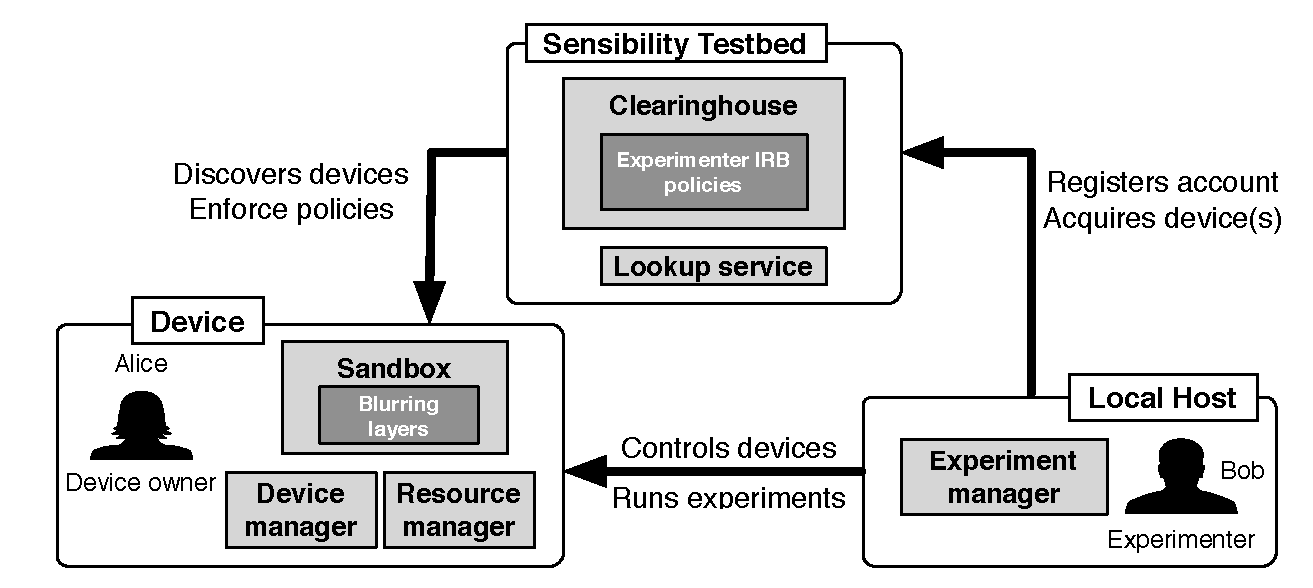
\includegraphics[width=\columnwidth]{figs/arch.pdf}}
%\vspace*{-20pt}
\caption{\small Sensibility Testbed architecture. \label{fig-arch}}
\end{figure}

\begin{table*}
\scriptsize
\centering

\bgroup
\def\arraystretch{1.15}% % for table padding
\begin{tabular}{|p{1.6cm}|p{1.6cm}|p{8cm}|p{3cm}|c|}
\hline
{\bf Goals\textsuperscript{*}}  & {\bf Sensor} & {\bf Sensor data} & {\bf Default 
policy\textsuperscript{\dag}} & {\bf Customizable} \\ \hline \hline

\multirow{3}{1.7cm}{\yanyan{?}} & \multirow{2}{*}{Battery} & Status (charging/discharging), temperature, 
 technology, health (good/overheat). & Full precision, or constant. & \multirow{2}{*}{\tickmark} \\ \cline{3-4}
 & & Battery level, voltage, plug-in type. & Round-up, or constant. &  \\ \cline{2-5} 
 
& Settings & Vibrate mode, screen settings (on/off, brightness, timeout), media/ringer 
volume. & Full precision, or constant. & \tickmark \\ \hline 

Prevent keyloggers. & Motion sensors & Accelerometer, gyroscope, magnetometer, orientation, ambient light. & Full precision, 
roundup, random rotation, or constant. & \tickmark \\ \hline 

\multirow{8}{1.7cm}{Prevent locating a device.} & \multirow{4}{*}{Location} & 
\multirow{3}{*}{Latitude, longitude, altitude.}  & Approximate to the nearest 
zipcode region, or city/state/country center. & \multirow{4}{*}{\tickmark} \\\cline{3-4}
%& & Speed. & Round-up, or constant. & \\\cline{3-4}
& & Location provider name (network/GPS/passive). & Full precision, or constant. & \\ \cline{2-5}

& \multirow{2}{*}{Cellular network} & Cell ID, neighboring cell ID(s). & Randomized ID. & N/A \\ \cline{3-5}
& & Network operator ID and name, country code, area code. & Hashed ID, names, 
and code. & \tickmark \\ \cline{2-5}

& \multirow{2}{*}{WiFi network} & WiFi connection information (router's SSID and MAC address). 
& \multirow{2}{3cm}{Hashed SSID, randomized MAC address.} & \multirow{2}{*}{\tickmark} 
\\ \cline{3-3}  
& & WiFi scan result (nearby WiFi routers' SSIDs and MAC addresses) & & \\ \hline 

\multirow{10}{1.7cm}{Prevent identifying a device owner.} & 
\multirow{3}{*}{Bluetooth} & MAC address.  & 
Randomized MAC address. & \multirow{2}{*}{N/A} \\ \cline{3-4}
 & & Local name, nearby Bluetooth device names. &
Hashed device names. &  \\ \cline{3-5}
 & & Scan mode, state (enabled/disabled). & Full precision, or constant. & 
 \tickmark \\ \cline{2-5}

& \multirow{3}{*}{Cellular network} & Roaming status, SIM card status (ready/absent), 
phone status (idle/busy), signal strength. & Full precision, or constant. & 
\multirow{2}{*}{\tickmark} \\ \cline{3-5}
& & Device ID, incoming number.  & Randomized ID and number. & N/A \\ \cline{2-5}

& \multirow{4}{*}{WiFi network} & WiFi connection information (Device MAC address, 
IP address, link speed, association state). & \multirow{4}{3cm}{Hashed IP address, 
randomized MAC address, full precision or constant frequency/signal strength.} & 
\multirow{4}{*}{\tickmark} \\ \cline{3-3}  
& & WiFi scan result (nearby WiFi routers' frequency, signal strength, 
security features). & & \\ \hline 

%Start/stop activities & & & \xmark \\ \hline 
%Running applications & & & \xmark \\ \hline 
\multirow{2}{1.7cm}{Prevent video/ audio recording.} & 
Camera & Take pictures, record videos. & \multirow{5}{*}{Disabled} & 
\multirow{5}{*}{N/A} \\ \cline{2-3} 

& Microphone & Voice record. & &\\ \cline{1-3} 

\multirow{2}{1.7cm}{Prevent actions for owner.}& Intent & Scan barcode, search, etc.  &  & \\ \cline{2-3} 

& Phone, SMS & Send/receive messages, delete messages, dial/pick up phone calls. & & \\  \cline{1-3} 

Protect owner's contacts. & Address book & Contact list of the device owner. & & \\ \hline 

\multicolumn{5}{l}{\textsuperscript{*}\scriptsize These goals are the common goals, though uncommon 
goals exist. For example, motion sensors can be used to fingerprint devices~\cite{bojinov2014mobile}, 
or record conversations~\cite{michalevsky2014gyrophone}.} \\ 

\multicolumn{5}{l}{\textsuperscript{\dag}\scriptsize As new threats emerge, we plan to adjust the default
policies.} \\ 

\end{tabular}
\egroup

\caption{\small Sensibility Testbed's default policies for controlling sensor data precision.
\yanyan{things like signal strength, mode, status should go to the first row.}}
\label{tab:default}
%\vspace{-10pt}
\end{table*}

%\subsubsection{Interacting Parties}\label{sec-parties}
The operation of Sensibility Testbed  involves three types of interacting
parties, as shown in Figure~\ref{fig-arch}: mobile \textit{devices} 
owned by ordinary people, with our app installed; a 
\textit{clearinghouse} server that discovers and configures
participating devices; and \textit{experimenters} who want to run
experiments on mobile devices. The interaction between these three 
components, as illustrated in Figure~\ref{fig-arch}, is designed to 
support three fundamental design principles.
%\subsubsection{Testbed Architecture}

\textbf{Shared access to device resources.} 
Since hardware resources are limited on mobile devices, it is 
not possible to dedicate an entire device to an experiment. Therefore, 
Sensibility Testbed allows several experiments to share one device. It 
uses a \textit{sandbox} to isolate one researcher's code from 
 another, through its performance isolation technique. The sandbox 
also prevents experiment code from inadvertently harming the device
via security isolation. Other software within the device includes a 
\textit{resource manager} that controls a researcher's access to a sandbox 
and allows the device to communicate with the rest of the testbed, 
and a \textit{device manager} that allows the device 
owner to opt in or out of the testbed. Together, they form the
\textit{device software} (Section~\ref{sec-repy}).

\textbf{Allocating devices and mediating data access.}
Sensibility Testbed is designed to provide both enhanced security and 
more efficient management of experimental setup, so another principle 
for the design was a central component that could serve as a a trusted 
intermediary for acquiring and managing device resources. Both tasks 
are delegated to  a server called \textit{clearinghouse}~\cite{ch}. The 
clearinghouse allows researchers to 
register accounts for each experiment, and share access to a common 
pool of devices, freeing them from the need to individually recruit participants. 
The clearinghouse can also allocate resources and mediate 
data access according to policies defined by a researcher's IRB. The 
clearinghouse thus facilitates device sharing and policy enforcement.  
Additionally, the clearinghouse uses a distributed service called 
\textit{lookup service} to keep track of the devices in the testbed 
(Section~\ref{sec-ch}).

\textbf{Local support for remote experimentation.} 
The last design principle was to allow researchers to manage their 
experiments on remote devices from a local machine, as is offered 
by other testbeds~\cite{hibler2008large, peterson2006experiences}. Sensibility 
Testbed addresses this need by using a tool called \textit{experiment 
manager}. The experiment manager provides access to 
hardware resources on mobile devices using the researcher's testbed 
credentials (assigned by the clearinghouse). This tool will be introduced
in Section~\ref{sec-emt}.

%\smallskip
%The following section describes %the three components in more detail, and 
%%addresses 
%how these parties interact to enable safe experimentation on mobile devices. 


\subsection{Policy Design}

The goal of \sysname is to protect the device owner's privacy, while making
the data from mobile devices useful for a wide range of research. \sysname
leverages a concept that not all sensors are alike. 
%As mentioned earlier, failure to recognize the vulnerability of
%certain sensors was a key reason for privacy breaches. 
In designing Sensibility Testbed, \textit{default policies} were set as 
to what types of sensors could be accessed, and the sensor data should be
accessed at which granularity or frequency to prevent common privacy and
security attacks. To privide such protection, \sysname 
%classifies sensors as 
%of low, moderate, or high risk. Sensors of high risk are not accessable to 
%researchers by default, and the sensors of low and moderate risk are further 
%protected by the default policies.
uses a set of policies to prevent a range of attacks, as listed in 
Table~\ref{tab:default}. These policies roughly fall into three categories.

\textbf{Category 1.}
First, the default policies disable cameras and microphones. The reason is 
that if a microphone is controlled by a malicious party, it can be used to 
intelligently choose data of a higher value, such as credit card number or 
password, to record~\cite{zhang2015leave}. Cameras face the same kind 
of risks. Meanwhile, the default policies disable interrupting actions, such as 
making phone calls, scanning a barcode on behalf of the device owner, 
and accessing an address book. 

\textbf{Category 2.}
Next, given our analysis of the current privacy attacks 
(Section~\ref{sec-our-policies}), identifying a device or its owner, locating 
a device, and inferring keys typed by a device owner are the most
common risks. In Table~\ref{tab:default}, sensor data like MAC address, 
device ID, etc., can be used to identify a device; latitude, longitude, cell 
IDs in a cellular network, a WiFi router's SSID can be use to locate a 
device; motion sensors like accelerometer and gyroscope can be used
as keyloggers to infer a credit card number or password typed on a 
smartphone. However, compared cameras and microphones, these 
sensors normally require a background process that continuously 
collects the data, or a sophisticated algorithm that constantly learns 
about the patterns of data generated. Therefore, the default policies 
blur these data, such as using randomized MAC addresses in a 
Bluetooth and WiFi network, approximated location coordinates, and 
slightly rotated motion sensor data. 

\textbf{Category 3.}
Finally, as long as the policies in the first two categories hold, research 
projects are allowed to get data at a level that is meaningful. For example, 
projects that are interested in monitoring human activity, wireless network 
performance, etc., sensor values are allowed to the granularity that is safe, 
as long as the device owers cannot be identified, located, etc. Some data 
can be accessed at full precision (cellular signal strength, WiFi link speed), 
whereas others have an upper bound on their access frequency. 
\yanyan{how to add frequency to the table?}

\begin{comment}
\textbf{Risk categorization.}
%Even if an IRB happened 
%to approve such a policy, there are certain sensors that the testbed's
%own IRB designates as off-limits due to the high risk associated with 
%potential breaches. 
%and for which access can be pre-approved with the
%researcher's local IRB. 
%Only those sensors listed on our project 
%wiki page~\cite{sensor-api} are accessible to a researcher. 
A summary of these sensors is listed in Table~\ref{tab:default}.
%with each one categorized as . 
%The list of sensors that Sensibility Testbed provides are all of moderate 
%to low privacy risks (marked by \tickmark), and the testbed further provides policy enforcement
%(Section~\ref{sec-policy}) to protect all the sensor data. Sensors 
%such as cameras and microphones that are deemed sensitive are not 
%exposed to experiment code by default (marked by \xmark). 
The classification into low, moderate or high 
privacy risk is motivated by the Android system, where 
permissions are categorized into different protection levels~\cite{level}:
\textit{normal} permissions are automatically granted to the apps, 
\textit{dangerous} permissions are given based upon the 
user's consent, and so on. In our case, 
%we divide sensors into different risk levels, as shown 
%in Table~\ref{tab:default}. 
%Sensors with low to moderate risk are 
%allowed and protected by IRB policies. Sensors of high risk are 
%disabled by default. 
we divide sensors into different risk levels by the consequences and 
difficulties of a potential attack. If a microphone is controlled by 
a malicious party, it can be used to intelligently choose data of a 
higher value (e.g., credit card number, password) to record~\cite{zhang2015leave}. On the other 
hand, in order to infer a credit card number or password typed on a 
smartphone using motion sensors, the attack requires the installation of 
a sophisticated algorithm on the device that constantly learns about  
the patterns of data generated by accelerometer or gyroscope. In contrast,
using battery information alone is not sufficient to create a fingerprint 
for each device. Different information and mutiple occurrences need to
be pieced together to extract this data~\cite{battery-priv}. Therefore, 
compared to motion sensors, a microphone is considered a higher risk, 
and a battery is a significantly lower risk.

\textbf{Default and customizable policies.}
For sensors of low and moderate risk, the default policies are listed in 
Table~\ref{tab:default}. Our principle to design the the default policies 
is that a device or its owner cannot be identifiable, but research projects
are allowed to get data at a level that is meaningful. For example, Bluetooth
and WiFi network MAC addresses can uniquely identify a device, therefore, 
the default policy for these sensor data is to return randomized MAC 
addresses to an experiment, as in~\cite{aditya2014encore}, and this is 
mandatory (marked by N/A). For research projects that are interested 
in monitoring human activity, wireless network performance, etc., sensor
values are allowed to the granularity that is safe. Some data can be 
accessed at full precision (cellular signal strength, WiFi link speed), 
whereas others have an upper bound on their access frequency. 
\yanyan{how to add frequency to the table?}

\end{comment}

The three categories of default policies serve as a common denominator 
to researchers' IRB policies. Researchers can further customize the policies 
with parameters that result in coarser data granularity. The default and 
customized policies are automatically enforced by the \sysname 
infrastructure. Such a 
protocol for research with mobile device sensors has been approved by
the IRB at New York University (IRB \# 15-10751). 
\cappos{Shouldn't this detail come earlier?  Why is this here instead?}

By default, risky sensor data is disabled or blurred. However, if such 
access is critical to the study, access must be requested by going through 
the \sysname IRB, in addition to the researcher's IRB. 
\yanyan{how to notify device owners policies changed?} 
\cappos{Don't you have some things you would never allow even if the NYU IRB
approves it?}
%\lois{following up on Yanyan's comment--If the Testbed's IRB says this expanded access is permissable, are the device owner's notified and can they opt out of this study? Otherwise, that would be a direct violation of the privacy protection you claim to give them}
%\lois{I did not touch these last two paragraphs because I still don't know about  the opt-out policy for individuals if this permission is given}
%Depending on the experiment description provided by the 
%researcher, the fields marked with a (*) are the ones that will be blurred.
%
%
%
As a result, Sensibility Testbed does not
provide unfettered access to all sensors. 
%Access to sensors of
%higher risk, e.g., the policies that request restricted sensor data, 
%or at higher frequencies than our default policies, 
%needs to go through the Sensibility Testbed's IRB,
%in addition to the researcher's IRB. 
In most cases, we expect
that researchers need only go through their local IRB to get
the sensor access they need for their experiment. 


\subsection{Testbed Operation}


The basic operation of Sensibility Testbed involves two separate 
parties: a device owner interested in participating in experiments 
and a researcher seeking to run tests on remote devices. The 
device owner starts by installing the Sensibility Testbed app from 
the Android app store~\cite{sensibility-app}, which includes all the 
device software (Section~\ref{sec-repy}). After downloading the app, 
the device owner is informed about the testbed's general usage policy 
in a consent form and must give consent before participating.
Any device owner, regardless of age, country, or background, can 
opt into our testbed in this manner, and can opt out just by uninstalling 
the app. The app will also display a list of experiments and each 
experiment's policies, so the owner can opt out of individual experiments. 

To conduct an experiment, a researcher will first provide his institution's 
IRB policies to the clearinghouse and will sign up for his experiment. \yanyan{need a screenshot} 
The clearinghouse server helps him acquire devices, and codifies 
policies specified by the researcher's IRB. After obtaining remote devices, 
the researcher can perform experiments directly on the devices through 
the experiment manager, using the credentials assigned by the clearinghouse. 



%Device owners like Alice participate in Sensibility Testbed by p.

%These policies restrict what and how data can be accessed by the 
%researcher. 
%into data blurring layers that are enforced on
%mobile devices. Such a process can protect device
%owners' personal information. 
%Researchers' code runs in a sandbox that isolates the code from the 
%rest of the device host system. 
%To control the execution of code, Bob uses his own 
%desktop or laptop computer to manage the 
%experiments via the experiment manager. It deploys 
%and runs experiments in sandboxes on remote devices that are 
%acquired through the clearinghouse.

%\textbf{Usage scenario 1: Smartphone owner volunteers as a testbed participant.}
%Alice downloads the Sensibility Testbed app from the Google Play 
%Store~\cite{sensibility-app}, which will install Repy and other software on her phone.
%The app displays a consent form, \yanyan{cite link} containing the testbed's 
%general usage policy. Alice must review and must agree to this 
%policy before installation. If Alice gives her consent, her device will be 
%installed with the Repy sandbox, the native Android code to 
%start or stop the sandbox, and an interface to communicate with the testbed 
%infrastructure (particularly the clearinghouse, described below). 
%By agreeing to our general usage policy, any device 
%owner, regardless of age, country, or background, need only to opt into our testbed as a
%volunteer \textit{once}, at the time of app installation. 
%%As a result, an 
%%researcher like Bob who wants to conduct an experiment 
%%%requests devices through our clearinghouse, which assigns 
%%%them devices from a set of available resources. As a result, 
%%%the researcher
%%does not need to get consent from each subject for each individual
%%experiment. \lois{is the previous sentence needed? I don't think so} 
%The testbed thus greatly simplifies the process for both the 
%device owners and experimenters. 

Two usage scenarios further illustrate how the clearinghouse 
protocol in operation, are given below. In this case, 
Alice, a device owner, participates in the testbed. A researcher, Bob, 
runs code on Sensibility Testbed using Alice's smartphone, discovered among other
devices. Specifically, Bob wants to know the cellular service
quality in major cities. As such, he needs location information
of individual devices, their cellular service provider, network
type (3G, 4G, LTE, etc.), and signal strength. 

\subsubsection{Clearinghouse tracks devices}\label{sec-case1}
Once the app is started, Alice's device can be discovered by 
the clearinghouse. The resource manager in her app periodically contacts 
a lookup service to advertise the device sandbox to the rest of the testbed, 
such as the clearinghouse or experiment manager. \yanyan{resource 
manager and lookup service have not been introduced yet.}
A lookup service is a distributed key-value store, such as a 
distributed hash table (DHT)~\cite{dht}, that allows one to associate 
keys with values and retrieve values associated with keys. In this case, 
Alice's resource manager uses an \textit{identification key}, \path{key.alice}, 
generated during the app installation, and associates this key 
with Alice's device IP address and port number, by 
storing this key-value entry in the lookup service. This key is not 
associated with Alice or her device's identity, but only with the app's 
installation on the device. 
%When the clearinghouse knows Alice's key, it can retrieve Alice's 
%IP:port by looking up her key, \path{key.alice}, through 
%the lookup service. With IP:port, the clearinghouse can then
%communicate with Alice's device over the network.
\yanyan{I think the device first puts key.sensibility 
in the lookup service. is this key's value key.alice? so when the 
clearinghouse looks up key.sensibility, it finds out key.alice; and then
it uses key.alice to lookup IP:port. But is it necessary to go into such detail?}

%The app interface also displays a list of experiment running
%on Alice's device, and their policies. Therefore, 
%through the app interface, Alice may uninstall, or 
%choose to opt out of individual experiments. 
%\lois{how? I have not seen this explained yet and I think its critical to discuss this}

To keep track of Alice's device, the
clearinghouse periodically queries the lookup service to
discover any new device installs. Once Alice's device is discovered, the
clearinghouse obtains \path{key.alice}, and thus
%clearinghouse uses a database that stores her device's unique
%identification key, \path{key.alice}, generated during installation. 
can retrieve Alice's  IP address and port number by 
looking up her key in the lookup service. This allows the clearinghouse
to communicate with Alice's device over the network.
If Alice uninstalls the Sensibility Testbed app, 
\path{key.alice} is deleted at the clearinghouse, which effectively unlinks
her device from any metadata stored on the clearinghouse. The key
will also be removed from the lookup service after a period of inactivity.
An experiment manager controlled by a researcher can lookup
available device installs in a similar way. Instead of finding all devices
available to the testbed, the experiment manager will only be able to 
lookup devices assigned to the researcher by the clearinghouse.

%The clearinghouse
%plays an intermediate role between the experimenter and 
%the device owner.
%As described in Section~\ref{sec-overview}, when an 
%experimenter registers at the clearinghouse, he
%needs to provide his IRB policies. These policies ensure that
%the researcher cannot conduct experiments to access data that
%extend beyond the experiment policy. The clearinghouse 
%translates and codifies each policy, and instructs the 
%sandboxes on remote devices to implement these policies. 
%When experiment code is running in the sandbox, the 
%policies will be applied to restrict %the precision of sensor 
%%data or the frequency to access 
%sensor access. 

\subsubsection{Researcher registers experiment and provides IRB policies}
\label{sec-case2}
 Researcher Bob's first step to access the testbed begins when he
%needs to provide a set of etailed IRB policies from his institution. 
%In order to obtain an IRB approval, a researcher first 
%To do this, Bob 
fills out an experiment registration form at the 
clearinghouse. The clearinghouse registration page shows 
a list of sensors accessible to testbed users, and 
each of their possible accuracy and access frequency limits. 
%\lois{I think I already asked this, but is it literally just the sensors that the page shows, and not the devices containing the sensors that are shown? It's a small point, but I think it has to be clarified} 
In this particular case, Bob specifies that 
%what data can be accessed by a research experiment, at which 
%granularity or frequency such data can be accessed, how data 
%should be securely stored, and so on. \yanyan{cite register 
%experiment website url.}
his experiment can (1) read location information
from devices at the granularity of a city, (2) read accurate
cellular signal strength and network type, as well as
%but not allow access to information about 
cell IDs, and (3) get location and
cellular network data updates every 10 minutes. 
%Bob submits an
%experiment description for these requirements, which the
%clearinghouse will codify into policies that are later enforced
%on remote mobile devices (Section~\ref{sec-ch}).
%Bob then uses this form, along with other forms downloaded 
%from the clearinghouse, to apply for IRB approval at his institution.
%
After filling out this form, Bob downloads the experiment description 
he provided, the detailed information about Sensibility Testbed and 
several relevant forms, such as 
those addressing consent, terms of participation (for device owners),  
terms of usage (for the researcher), and so on. \yanyan{cite our docs}  
Bob then uses these forms as a template to complete the IRB application 
with his institution. These forms serve as a set of reference documents 
to make it easier for researchers like Bob to 
file the necessary IRB paperwork with their institutions.

After the application is submitted, Bob's IRB may disagree with 
his initial experiment requirements. For example, Bob's IRB will not permit
his experiment to access cell IDs in cellular networks, but 
approves the other policies. 
%Bob wants to access cell 
%IDs in cellular networks, but his IRB disallows such data access. Bob then
In this case, Bob will revise the experiment registration form, refile the paperwork, 
and obtain IRB approval. Bob then submits the revised  
registration form and his IRB approval to the clearinghouse.

Finally, the clearinghouse
parses Bob's registration form, extracts each data accuracy and access 
frequency limits approved by Bob's IRB policies (to blur an exact location 
to a city center, disallow access to cell IDs, and allow cellular network and 
location query once every 10 minutes), and assigns an experiment 
account to Bob. Once his account is activated, 
%Bob obtains his \textit{authentication keys} assigned by the 
%clearinghouse. These keys are to authenticate Bob with the 
%clearinghouse and the set of devices to which he has access.
%\path{bob.public} and \path{bob.private}. Next, 
Bob obtains his public/private key pair, and can request a number of devices from the 
clearinghouse (Section~\ref{sec-ch}). The clearinghouse then looks up
available devices like in Section~\ref{sec-case1}. If the clearinghouse 
discovers that Alice's device is available, it
assigns her device to Bob's experiment account by placing Bob's
public key in Alice's sandbox. At this point, Bob can remotely access Alice's 
device through his experiment manager and can stop and start the experiment.

As already described, the clearinghouse has a default set of blurring layers 
for accuracy and access frequency levels for each sensor. 
The clearinghouse first instructs 
the sandbox on Alice's device to add Bob's policies by preloading
a set of blurring layer code. It then supplies the extracted data from 
Bob's registration form as input parameters to the blurring layers. 
%that will be instantiated on Alice's device. 
When Bob runs his experiment, the policies are transparently applied
to the experiment code. 
The policies are easily customizable. Details about
how policies are implemented will be introduced in Section~\ref{sec-policy}.

%\textbf{Usage scenario 4: Researcher acquires device(s) and runs an experiment.}
%\label{sec-acquire-run}
%The above clearinghouse protocol ensures the enforcement of data
%access policies. Additionally, 
%To perform an experiment, Bob needs to request the use of some devices. 
%Recall that a testbed-specific key, \path{key.sensibility}, is distributed
%with the Sensibility Testbed app downloaded and installed by device
%owners (Section~\ref{sec-owner-participate}). 
%
%\yanyan{Albert thinks this is too much detail.}
%At this moment,  Bob has obtained an account with the clearinghouse.
%and is assigned a pair of public and 
%private keys, \path{key.bob-pub} and \path{key.bob-priv}, by the
%clearinghouse. 
%If the clearinghouse finds that Alice's device is available from the 
%lookup service, it
%%adds Bob's public key, \path{key.bob-pub}, to
%%the sandbox on Alice's device. This indicates that Bob is
%%authorized to use this sandbox on Alice's device, and 
%assigns Alice's device to Bob's experiment account by placing Bob's
%public key on Alice's device. It then instructs 
%the sandbox on Alice's device to add Bob's policies by preloading
%a set of blurring layer code. At this point, Bob can access Alice's 
%device through the experiment manager, just like using \texttt{ssh}.
%Bob writes his experiment 
%code in the Python-like language supported by our secure sandbox.
%The following is a snipet of code that gets location coordinates 
%from a device:
